\documentclass[11pt,letterpaper]{article}
\usepackage[margin=1in]{geometry}
\usepackage{graphicx}
\usepackage{hyperref}
\usepackage{listings}
\pagestyle{headings}
\usepackage{epstopdf}

\begin{document}

\title{PHY 410 \\ Homework Assignment 1}
\author{Han Wen \\ \tiny Person No. 50096432}
\date{\today}

\maketitle

\begin{abstract}
The goal of this assignment was to use numerical method to analyse some astronomical data to obtain Hubble's constant from various ways.
\end{abstract}

\tableofcontents

\newpage
\section{Problem 1}

\subsection{Hubble's Discovery}

Edwin Hubble published his results on cosmological expansion in
a 1929 article\cite{hubble1929}.
His data are summarized in Fig.~\ref{figure1} and Table~\ref{table1}

\begin{figure}
\begin{center}
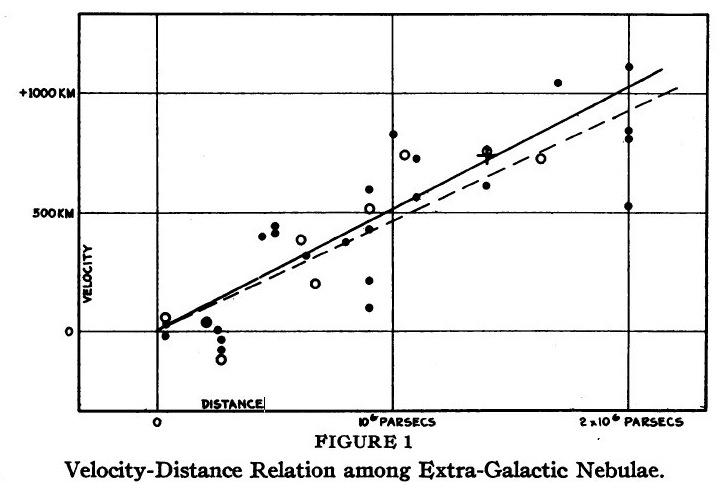
\includegraphics[width=0.9\linewidth]{hubble-fig1.png}
\caption{From Hubble's article\cite{hubble1929}.}
\label{figure1}
\end{center}
\end{figure}



\subsection{Numerical Analysis}

\begin{equation}
rK + X\cos\alpha\cos\delta + Y\sin\alpha\cos\delta + Z\sin\delta = v
\label{hubble-equation}
\end{equation}

Eq. \ref{hubble-equation} was simplified
\[
v = a+br
\]


Today we are going to reproduce the numerical analysis using python script with both the case of all data and the 9 groups method. As you can already see, the data has already been sorted into 9 groups based on the distance and the direction. The mechanism of the distribution is to first divide them into 3 groups with first the distance ranges from 0.032 to 0.5, the second from 0.5 to 1.0 and the third from 1.1 to 2.0. Then, according the their declinations, divide each group into 3 sub groups making totally 9 groups. Using the average distance and velocity of each group as shown in Table~\ref{table2}

\newpage
\begin{table}
\begin{center}
\begin{tabular}{|c|c|c|c|c|c|}
\hline\hline
Name & A(hours:minutes) &  D(degrees:minutes)&  $r$ (Mpc) &  $v$ (km/s) & group\\
\hline\hline
\input pro1table.tex
\hline\hline
\end{tabular}
\caption{Hubble's data}
\label{table1}
\end{center}
\end{table}

\begin{table}
\begin{center}
\begin{tabular}{|c|c|c|}
\hline\hline
Group Number & Distance $r$ (Mpc) & Radial velocity $v$ (km/s) \\
\hline\hline
\input groupdata.tex
\hline\hline
\end{tabular}
\caption{Hubble's 9 groups data}
\label{table2}
\end{center}
\end{table}

\subsection{Results}

\begin{figure}
\begin{center}
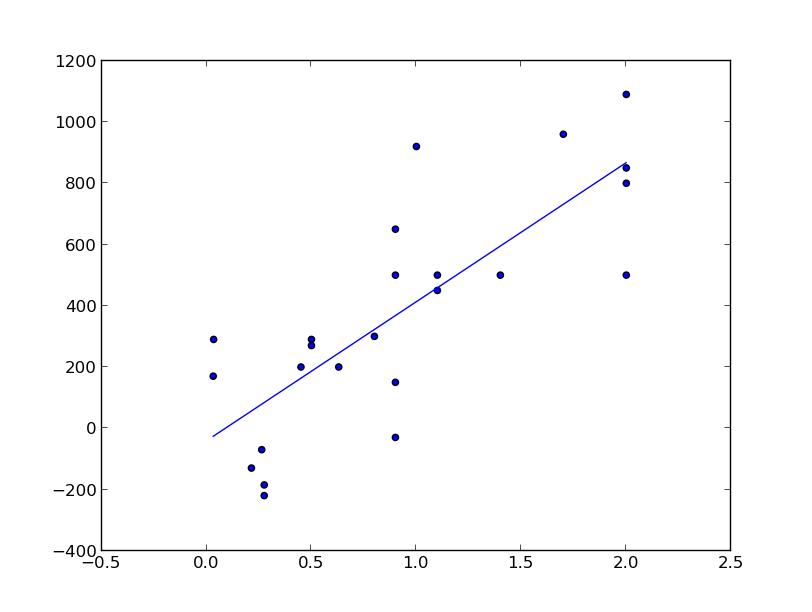
\includegraphics[width=0.6\linewidth,angle=0]{all.png}
\caption{The output using all the data.}
\label{figure2}
\end{center}
\end{figure}

\begin{figure}
\begin{center}
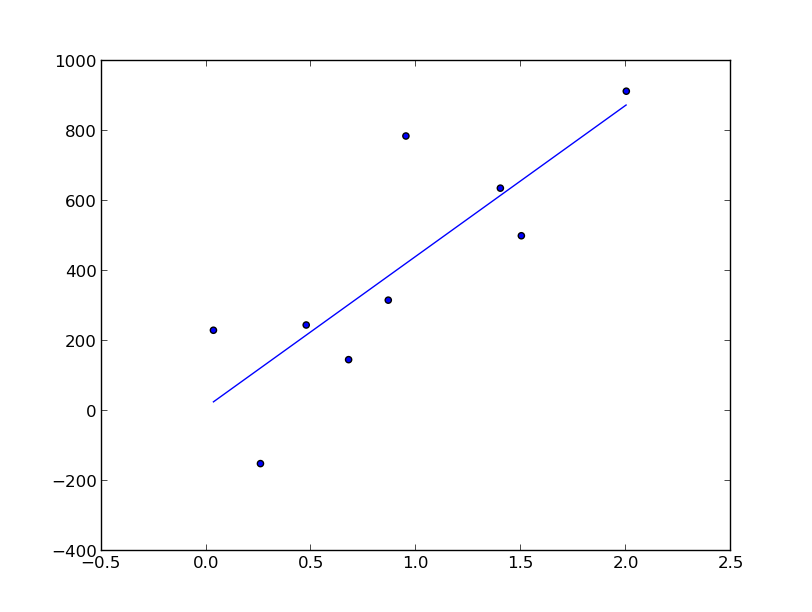
\includegraphics[width=0.6\linewidth,angle=0]{group.png}
\caption{The result using 9 groups data.}
\label{figure3}
\end{center}
\end{figure}

Using all the data, a=$-40.78 \pm 83.44$ Km/s and b=$454.16 \pm 75.24$ Km/s/Mpc, and the output plot is here ~\ref{figure2}

Using the 9 groups data, a=$11.21 \pm 126.59$ Km/s and b=$431.37 \pm 116.58$ Km/s/Mpc, and the output plot is here ~\ref{figure3} 

Since the age of the universe is 1/Hubble's constant \cite{hubblewiki} , I have the age of the universe is $215 \pm 36\times10^7 yrs$ for all data method and $227 \pm 61\times10^7 yrs$ for nine groups method.

\newpage
\section{Problem 2}
\subsection{Supernovae}
Find Hubble's constant from the intercept and slope output of the supernova program and compare with Hubble's value. Explain any discrepancies you observe.

\subsection{Numerical Analysis}
As with the supernovae, it no longer obeys the simple non-relativistic form of the Hubble's law:$v=rK+const$, the relativistic form must be employed:
$$
\mu=25+5log_{10}(\frac{cz}{H_o})+1.086(1-q_0)z+...
$$
Considering $q_0=0$ in our case, the equation can be written as:
$$
\mu=25+5log_{10}(\frac{c}{H_o})+5log_{10}z
$$
Therefore we can calculate the $H_o$ by means of the linear relationship between $\mu$ and $log_{10}z$,namely the intercept $I$and$H_o$can be linked by:
$$
I=25+5log_{10}(\frac{c}{H_o})
$$ 
So$H_o=\frac{c}{10^{{I/5}-5}}$

\subsection{result}

\begin{figure}
\begin{center}
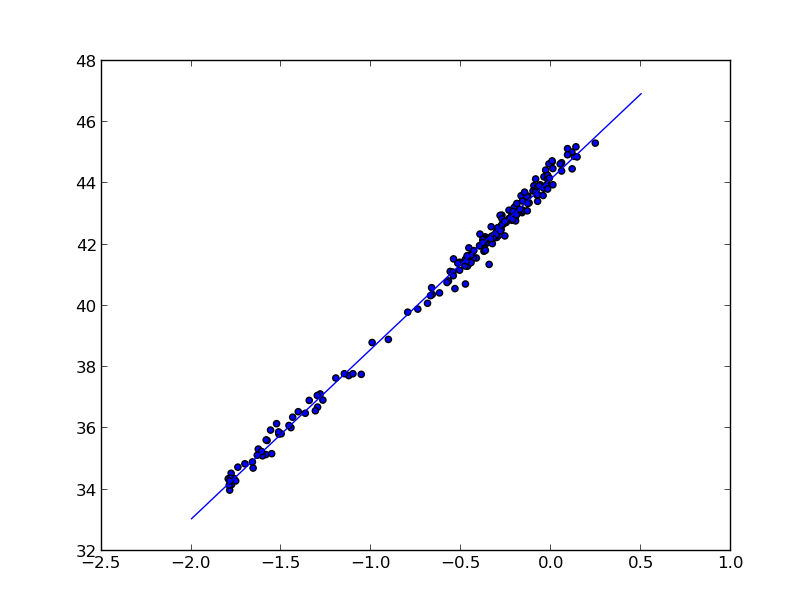
\includegraphics[width=0.6\linewidth,angle=0]{supernovaall.png}
\caption{The output using supernovae using all the data.}
\label{figure4}
\end{center}
\end{figure}

The linear fits result is shown in picture ~\ref{figure4}.
The slope is $5.553\pm0.026$ and the intercept is $44.152\pm0.022$
Correspondingly, the Hubble's constant is $H_o=44.329km/s/Mpc$

\newpage
\section{Problem 3}
\subsection{LOW AND HIGH RED SHIFT}
Divide the supernova data set into two subsets, low redshift and high redshift. Compute the slope separately for each of the two subsets. Can you conclude from your results that the expansion of the Universe is constant, accelerating, or decelerating?
\subsection{Numerical analysis} 
Based on z values we can divide data into two groups, one with z smaller than 0.7 and those larger than that.
To achieve that, I added some extra lines in the python script to write those two files.
\subsection{result}

\begin{figure}
\begin{center}
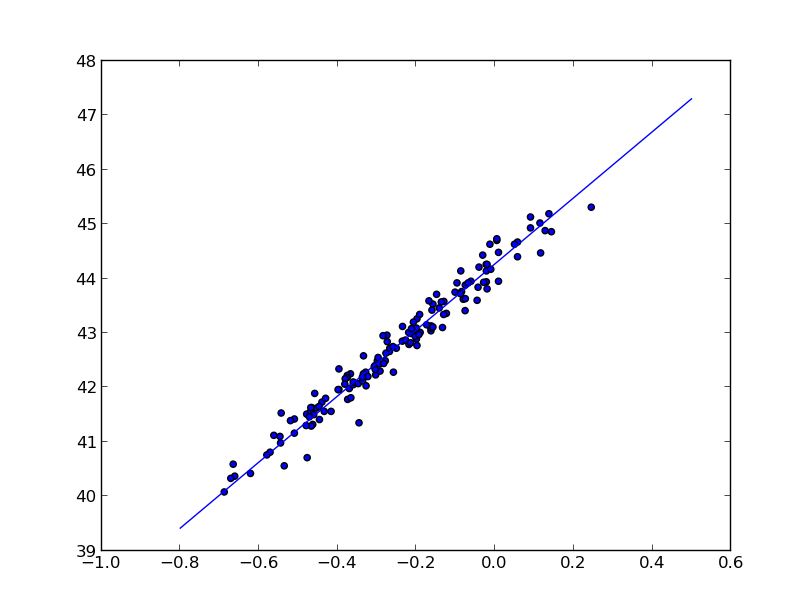
\includegraphics[width=0.6\linewidth,angle=0]{supernovagt7.png}
\caption{The output using supernovae using high shift the data.}
\label{figure5}
\end{center}
\end{figure}

\begin{figure}
\begin{center}
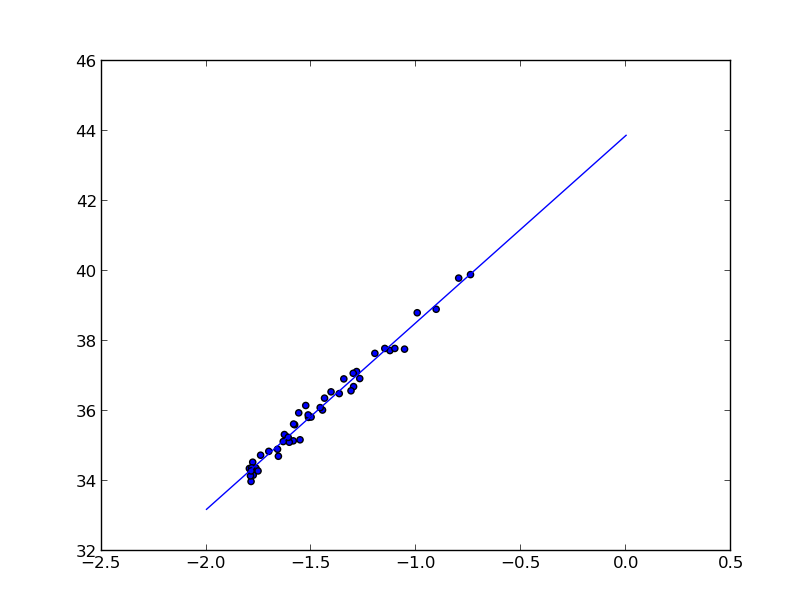
\includegraphics[width=0.6\linewidth,angle=0]{supernovast7.png}
\caption{The output using supernovae using low shift the data.}
\label{figure6}
\end{center}
\end{figure}

For the group with high shift~\ref{figure5}, we have The slope is $6.070\pm0.098$ and the intercept is $44.272\pm0.031$
Correspondingly, the Hubble's constant is $H_o=41.952km/s/Mpc$.

For the group with low shift~\ref{figure6}, we have The slope is $5.346\pm0.105$ and the intercept is $43.875\pm0.153$.
Correspondingly, the Hubble's constant is $H_o=50.363km/s/Mpc$.

Based on the result above, the expansion of the universe is increasing.


\newpage
\section*{Acknowledgements}

I discussed this assignment with my classmates and used material from the
cited references, but this writeup is my own.

\begin{thebibliography}{9}

\bibitem{hubble1929}
``A Relation Between Distance and Radial Velocity Among Extra-Galactic Nebulae'',
Edwin Hubble, Proc. Natl. Acad. Sci. USA {\bf 15}, 168-173 (1929).

\bibitem{coursepage}
PHY 410-505 Webpage, \url{http://www.physics.buffalo.edu/phy410-505}.

\bibitem{hubblewiki}
Wikipedia:Age of the universe,\url{http://en.wikipedia.org/wiki/Age_of_the_universe}.

\end{thebibliography}

\newpage
\appendix
\section{Appendix}

\subsection{python code}

The following python code was used to obtain the results in this report:

\lstinputlisting[language=python]{hubble_all.py}

\lstinputlisting[language=python]{supernovaall.py}

\end{document}
